This section gives a formal specification of our system. Our class diagram has some redundant links in it, which made the specification much harder. When we figured out why some of our predicates were invalid, we didn't have time to change the model anymore, so we tried deep comparing instead of normal comparing.

An example of this is the \texttt{addResponse} predicate. We wanted to specify that the new set of responses was the old set of responses unioned with a singleton containing the new response, but because of the links in Response, User and Event, this was not possible.

\subsection{Sigs}
	\subsubsection{Core module}
		This is our core module. Because of some of the predicates, all sigs have to be in here, except for DateTimeSlot.
	
		\lstinputlisting{alloy/Core.als}
	
	\subsubsection{DateTimeSlot}
	
		\lstinputlisting{alloy/DateTimeSlot.als}
	
\subsection{Facts}
	All facts about the core are in one module, factsCore.
	
	\lstinputlisting{alloy/factsCore.als}
	
\subsection{Preds}
	\subsection{Show the core}
		A trivial predicate to show everything.
		
		\lstinputlisting{alloy/predShowCore.als}
		
	\subsection{Event}
		Some predicates for the Event sig.
		
		\lstinputlisting{alloy/predsEvent.als}
		
	\subsection{Poll}
		Some predicates for the Poll sig.
		
		\lstinputlisting{alloy/predsPoll.als}
		
\subsection{Trace}
	The following images give a trace of our specification.
	
	\subsubsection{Core}
		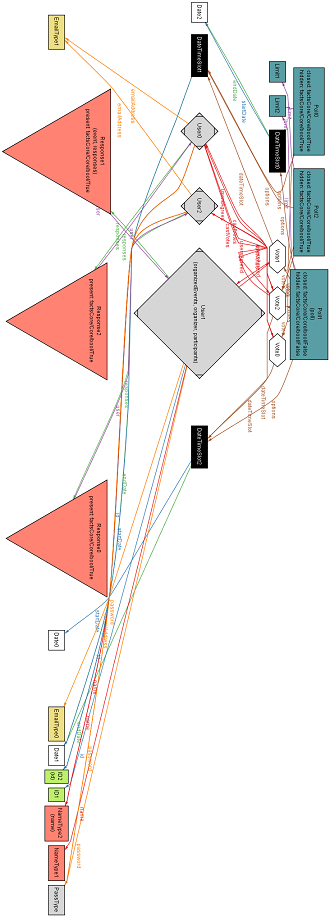
\includegraphics[width=\linewidth]{alloy/trace/show.png}
		
	\subsection{Open Poll}
		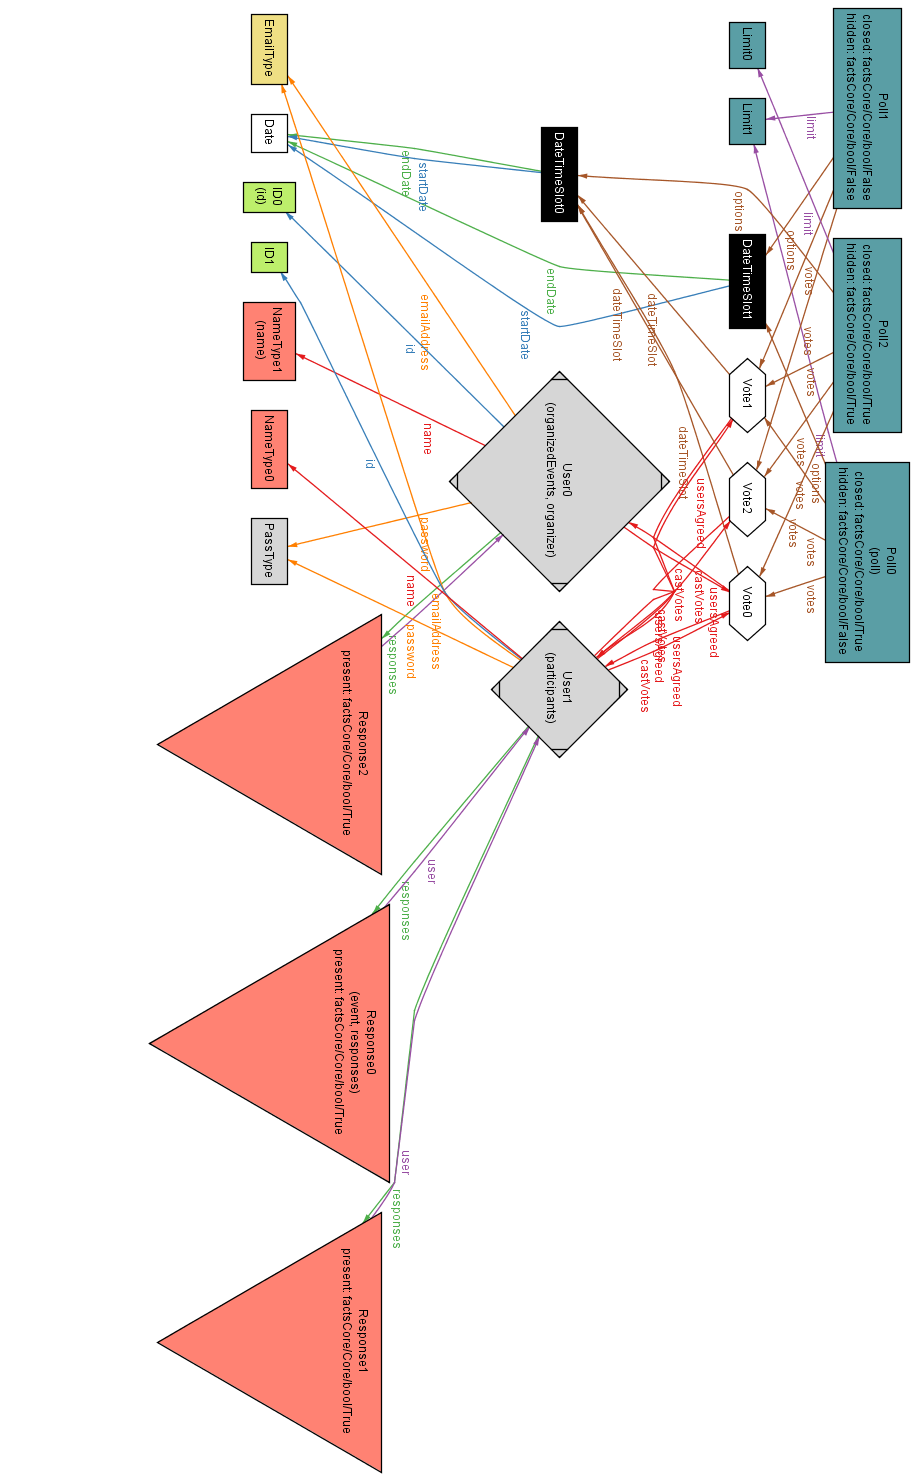
\includegraphics[width=\linewidth]{alloy/trace/poll1.png}
		
		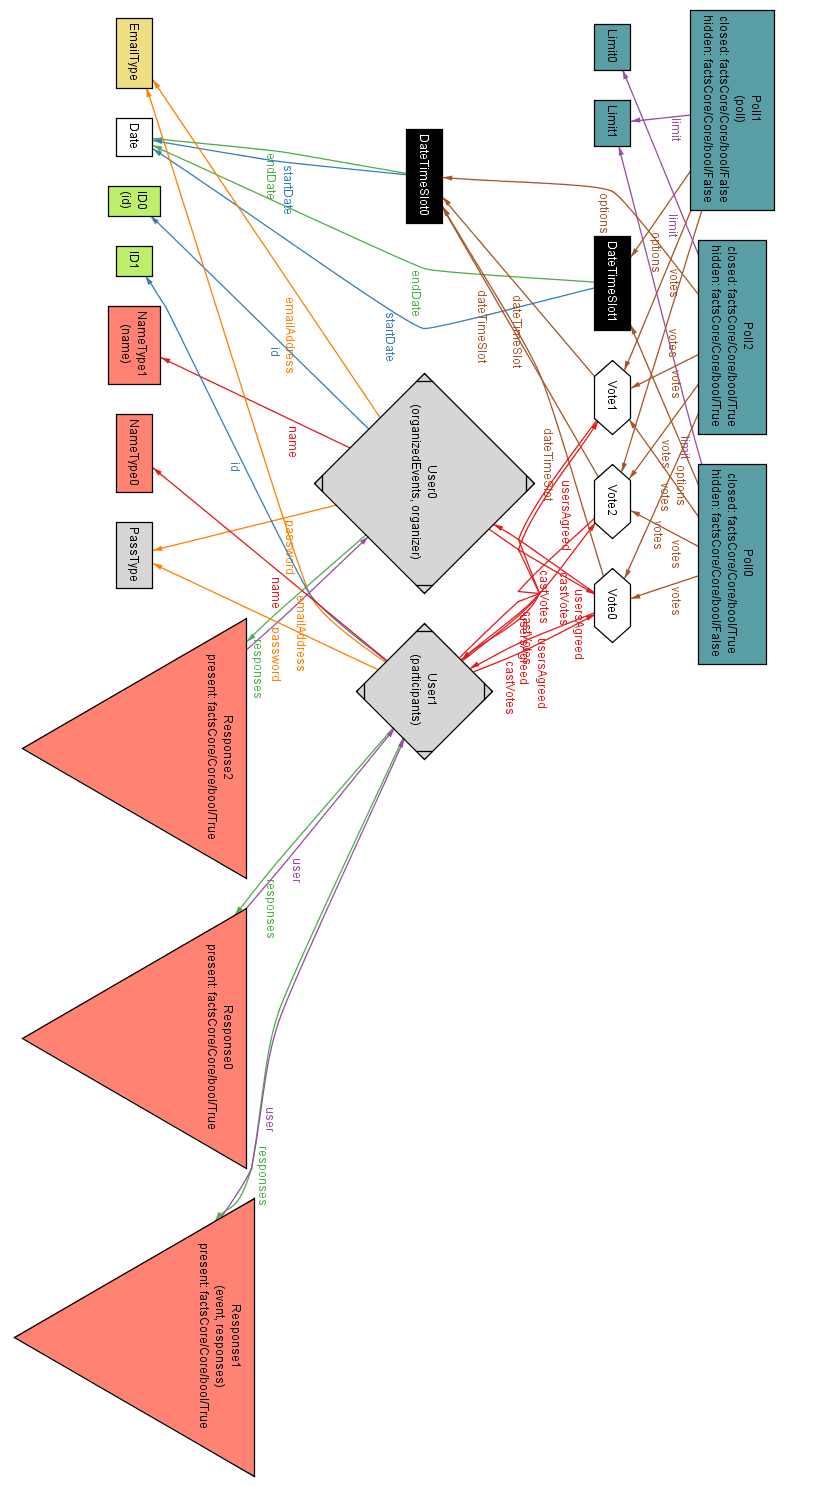
\includegraphics[width=\linewidth]{alloy/trace/poll2.png}
		
	\subsection{Adding vote}
		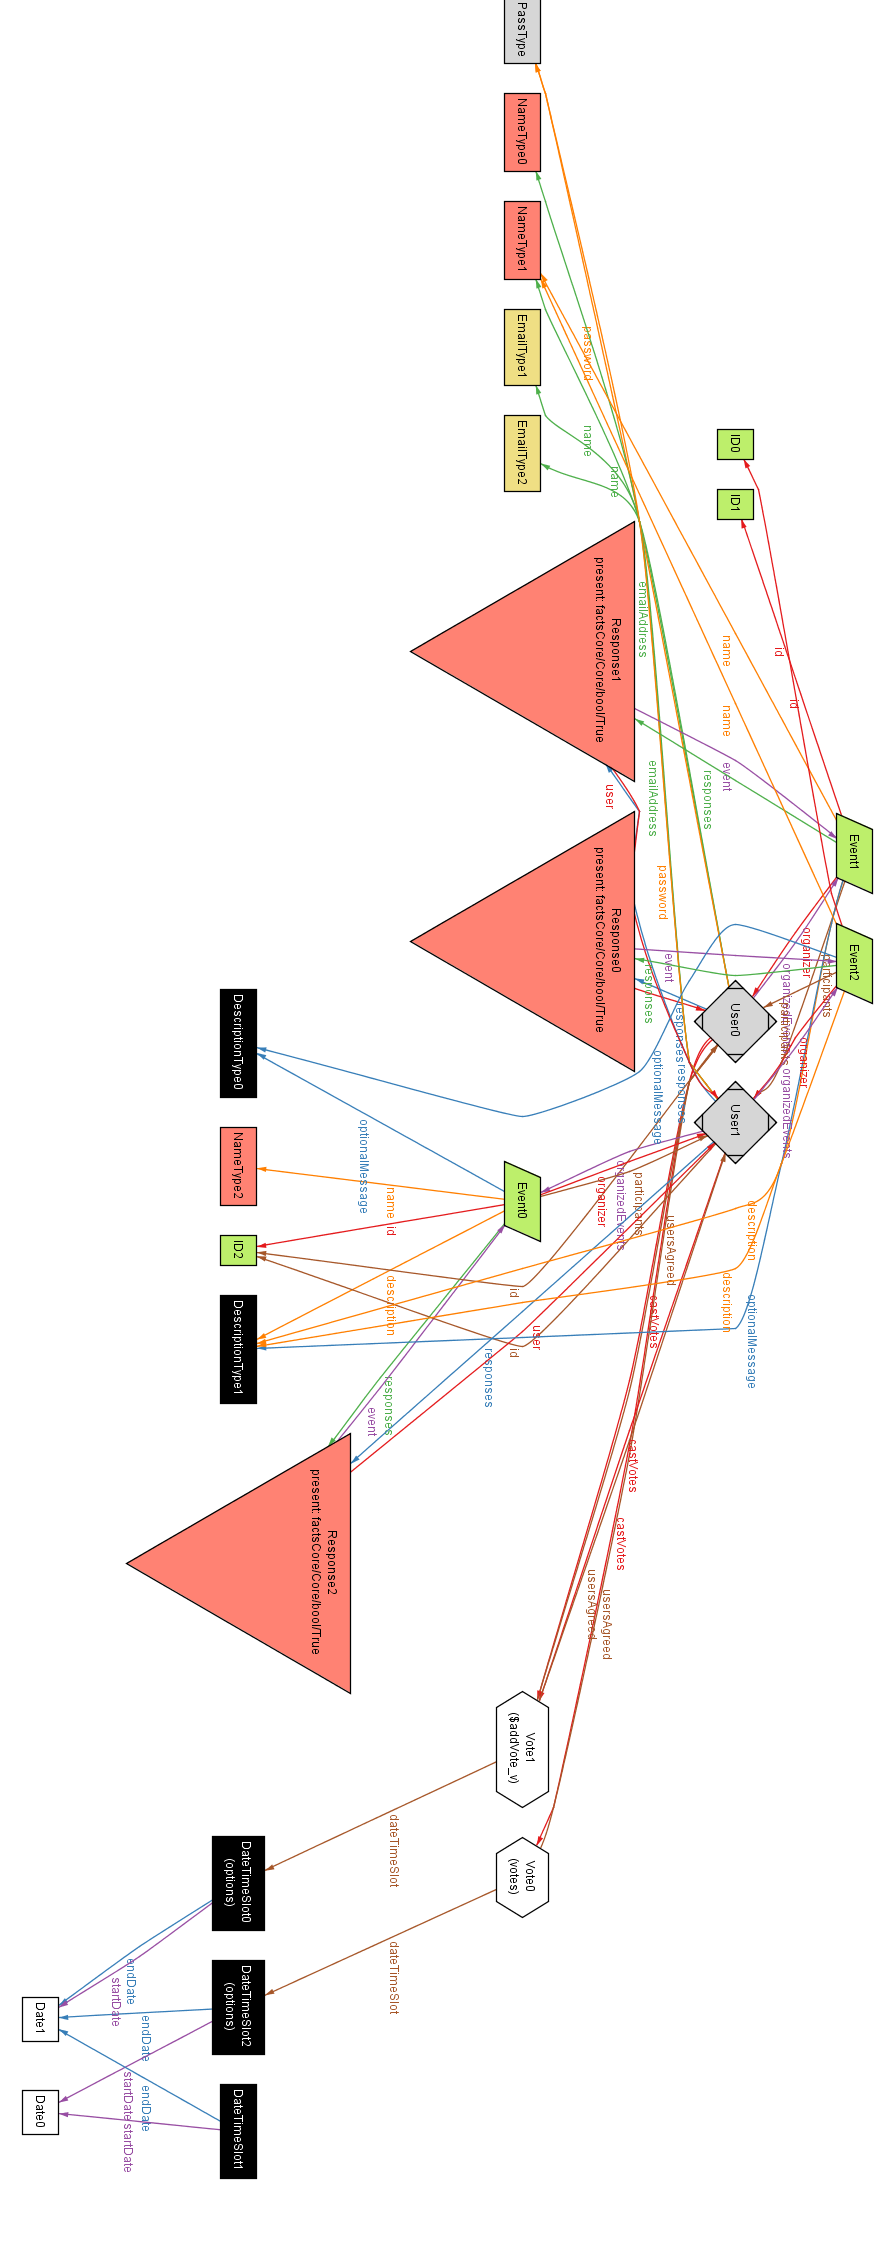
\includegraphics[width=\linewidth]{alloy/trace/vote1.png}
		
		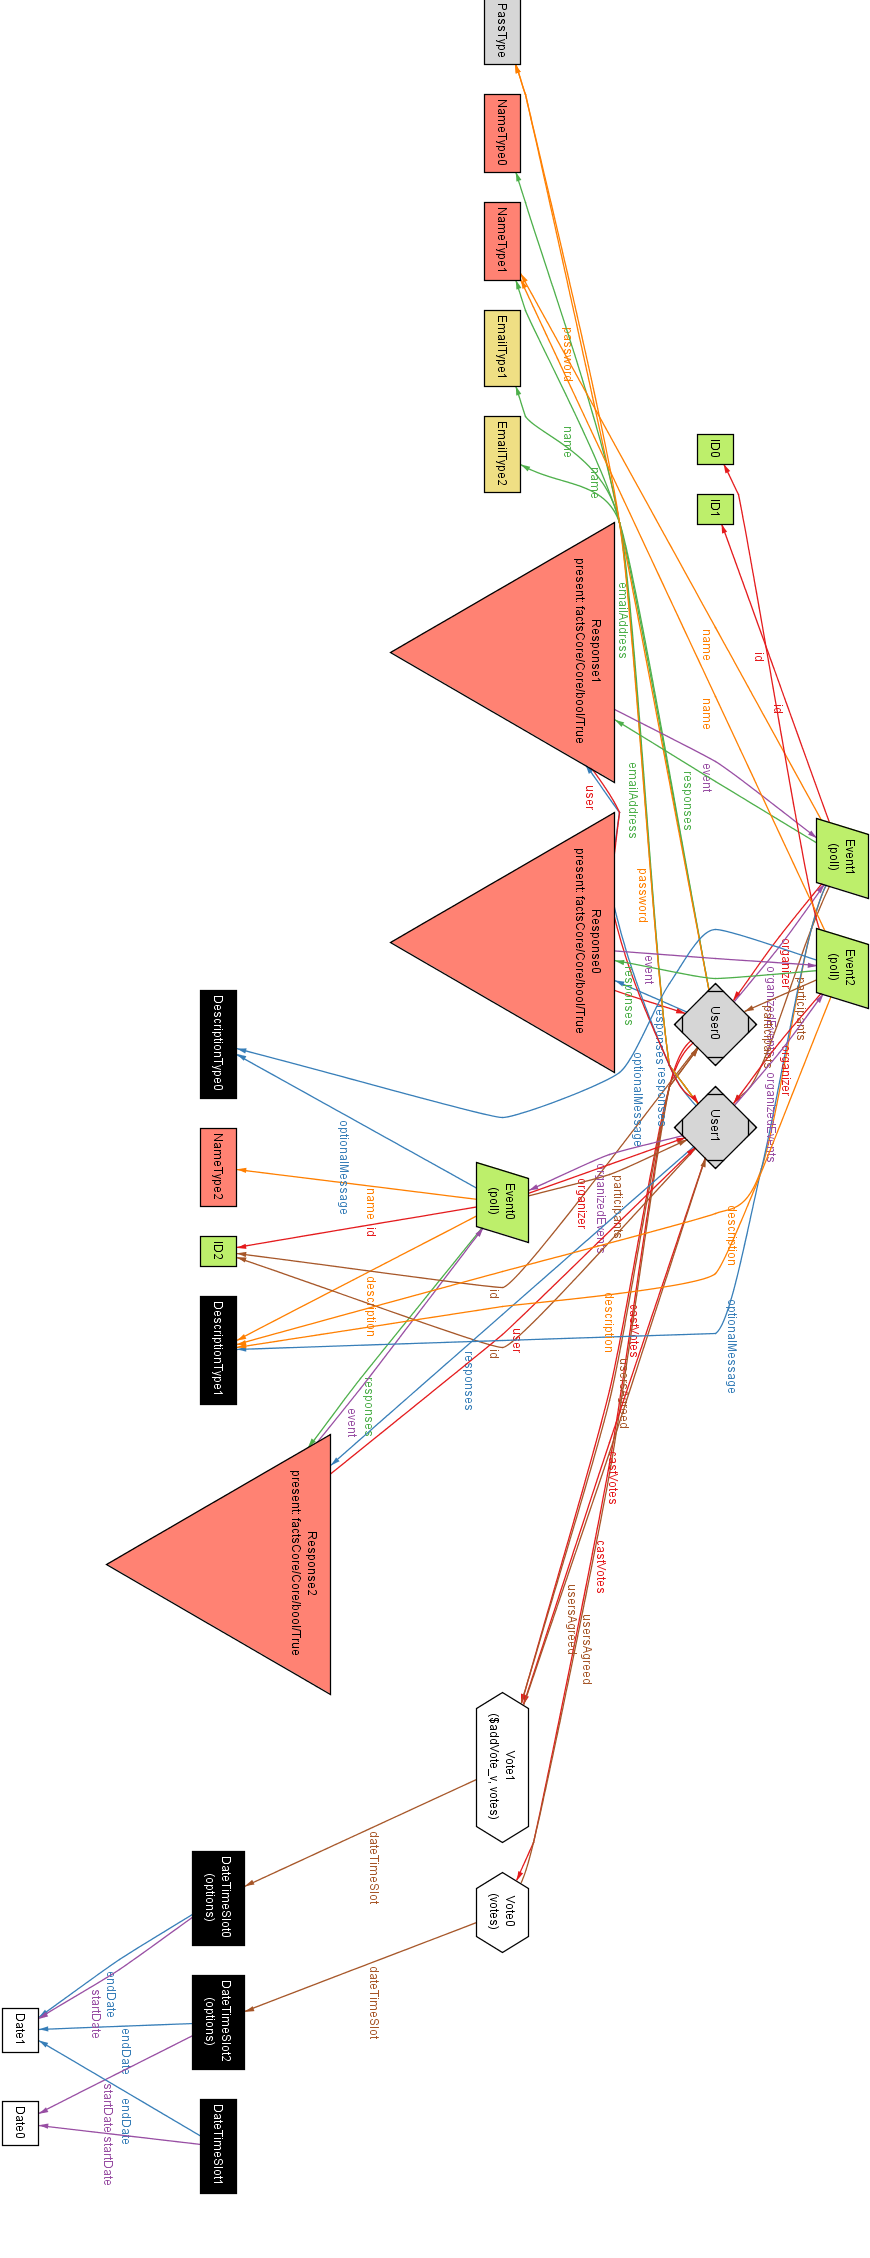
\includegraphics[width=\linewidth]{alloy/trace/vote2.png}
	
\subsection{Get the specification}
	To download this complete set of files, you can clone our git repository at \texttt{git://github.com/timvdalen/2IW05-project.git}. You can also browse the code online at \url{https://github.com/timvdalen/2IW05-project/tree/master/alloy}.
